Partimos de la base de que, como se ha comentado anteiormente, somos una empresa a la que se la ha adjudicado el despliegue de infraestructura de red 4G con el objetivo de prestar servicio a vehículos conectados. Dicho servicio queremos que se implemente en la autovía que conecta la ciudad de Salamanca con Tordesillas, en Castilla y León. \\

El tramo de carretera seleccionado comprende 73 kilómetros, en concreto desde el kilómetro 158 al kilómetro 231 de la A-62. En dicho tramo nos encontramos con que ya existe una buena infraestructura de red 4G prestando servicio, por ello vamos a aprovechar parte de ella. En concreto, haremos uso de las torres de telefonía ya disponibles, disponemos de 11 a lo largo de la carretera, tal y como podemos observar en la figura \ref{autovia}. En las torres que sean necesarias (que no tienen por qué ser todas) instalaremos nuestros propios equipos, como estaciones base y antenas. Es importante evaluar cuidadosamente los costes asociados a los componentes y considerar opciones con precios competitivos. \\


\begin{figure}[H]
    \centering
 	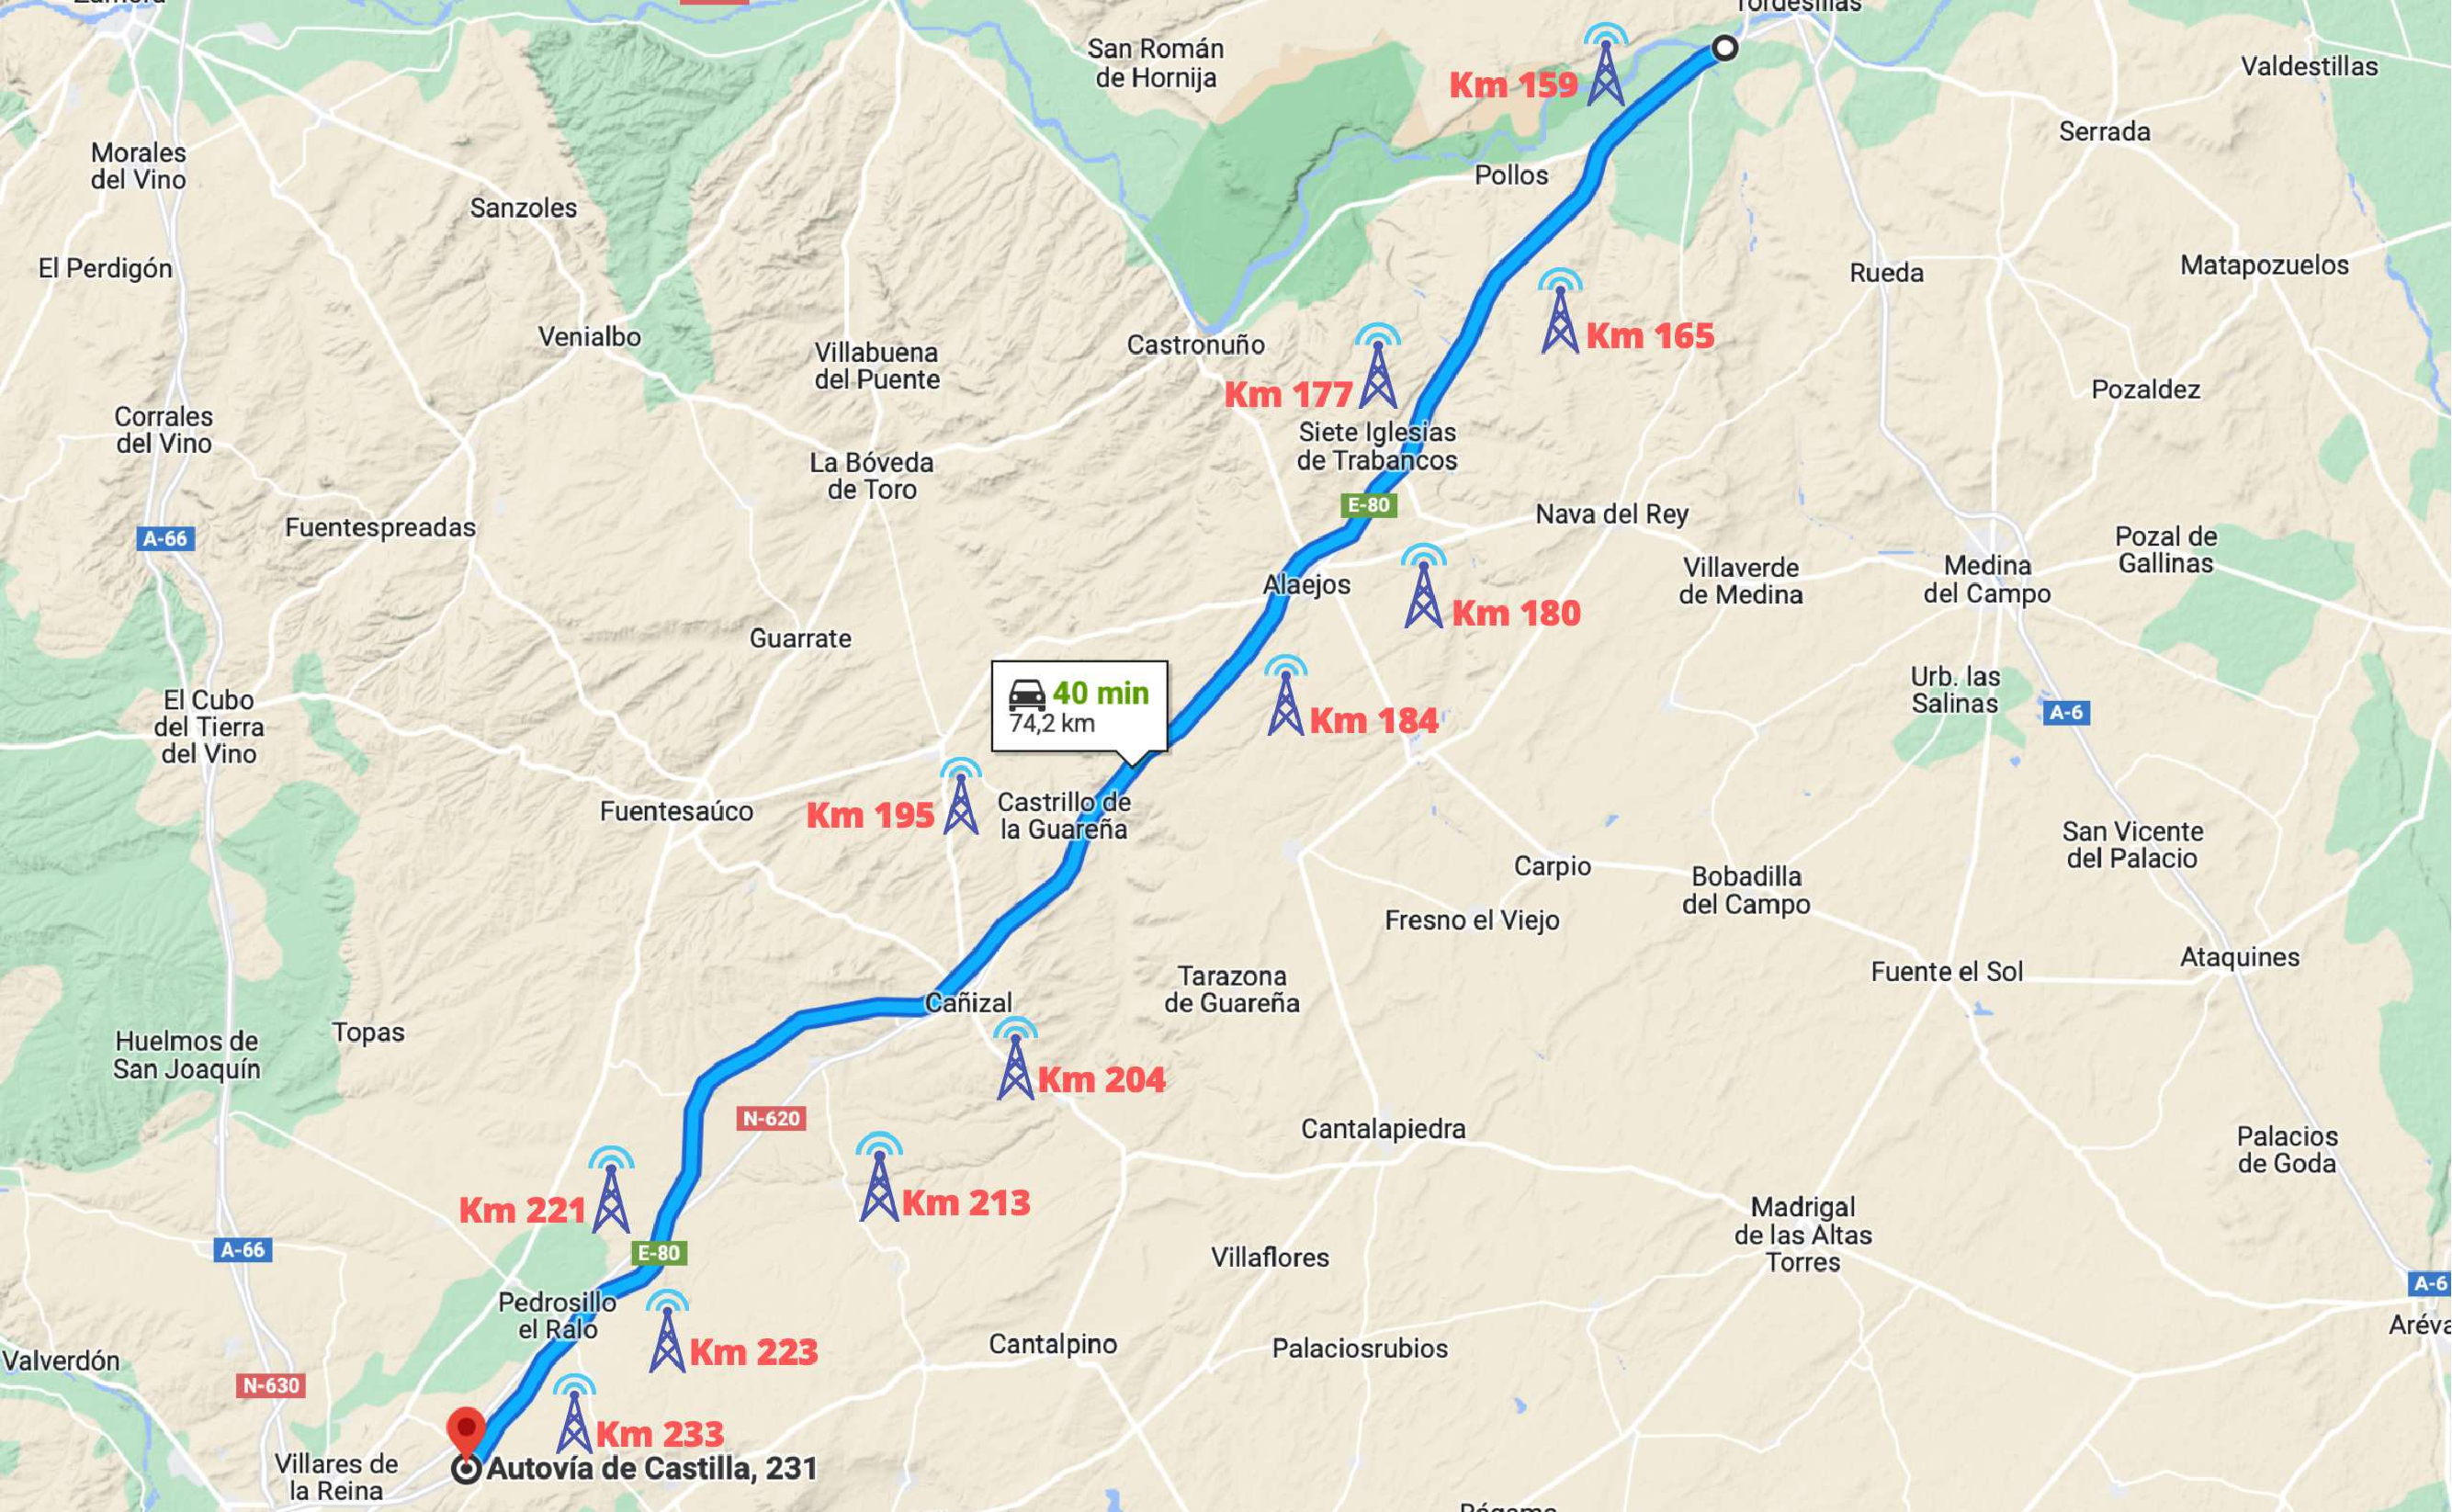
\includegraphics[width=\textwidth]{Imagenes/PlanteamientoInicial/torres_telefonia.pdf}
    \caption{Mapa de la autovía A-62 y las torres de comunicación existentes }
    \label{autovia}
\end{figure}

Queremos que un número elevado de coches pueda hacer uso de dicho servicio de manera ininterrumpida, es decir, que cada coche tenga capacidad suficiente para enviar el vídeo captado por la cámara durante todo el recorrido. Por eso, es necesario disponer de un ancho de banda de al menos varios Mbps, todo dependiendo de la calidad del vídeo que queramos ofrecer. \\

Prestando este servicio, los vehículos de los usuarios tendrán la capacidad de detectar las señales de tráfico aumentando así la seguridad vial, ya que así los vehículos pueden adaptar su velocidad y comportamiento en la carretera, lo que puede reducir el riesgo de accidentes y mejorar la seguridad en general. De igual forma, puede fomentar el cumplimiento de las normativas y regulaciones de tráfico, disminuir la cantidad de sanciones, o puede ayudar a optimizar el consumo de combustible y moderar las emisiones de gases contaminantes procedentes de dichos vehículos.\\

La seguridad en las carreteras es uno de los temas más importantes en el mundo actual. Una de las medidas para garantizar la seguridad es la señalización vial, la cual indica a los conductores las condiciones y normas de circulación. Sin embargo, a menudo las señales pueden ser difíciles de identificar debido a factores como su ubicación, desconocimiento de la misma o la distracción del conductor.\\

Para resolver este problema, se puede utilizar el aprendizaje automático para diseñar modelos capaces de detectar de manera precisa y eficiente las señales de tráfico. Estos modelos pueden ayudar a mejorar la seguridad en las carreteras permitiendo que los conductores reciban información clara y precisa en todo momento.\\

En este contexto, nuestra empresa ha sido encargada de diseñar e implementar un modelo de aprendizaje automático para la detección de señales de tráfico. Para eso, debemos utilizar técnicas avanzadas de procesamiento de imágenes. El objetivo final es contribuir a la seguridad en las carreteras y ofrecer soluciones innovadoras y eficaces.\\

Con el objetivo de poder prestar dicho servicio, se debe elegir qué modelo de inteligencia artificial se va a seleccionar para llevarlo a cabo. En el campo de la detección de objetos en imágenes y vídeos, existen varios modelos de aprendizaje automático que se pueden utilizar. Uno de los más avanzados y precisos es YOLO. Lo que le distingue de otros modelos es su capacidad para detectar múltiples objetos en una sola imagen de manera eficiente y precisa, utilizando redes neuronales convolucionales (CNN) y técnicas de filtrado de cajas delimitadoras. \\

